\begin{TP}[À l'assaut des carrés magiques !]

\vspace{1em}\textbf{1\up{ère} Partie : Le principe}\vspace{1em}

\item Voici un carré magique d'ordre 3. \og Être magique \fg suppose que la somme des nombres en ligne, en colonne et en diagonale soit la même. Vérifiez que ce carré est bien magique.

\vspace{1em}

\begin{center}
    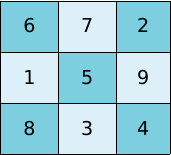
\includegraphics[width=.15\linewidth]{EqEA03}
\end{center}

\vspace{1em}

Voici une méthode pour construire des carrés magiques d'ordre 4 :

\vspace{1em}

\begin{center}
    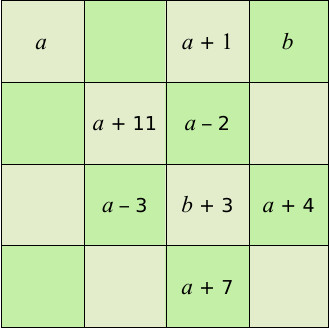
\includegraphics[width=.35\linewidth]{EqEA04}
\end{center}

\vspace{1em}

\item Soit $S$ la somme commune aux lignes, aux colonnes et aux diagonales. Exprimez $S$ en fonction de $a$ et de $b$.
\item\label{EQtp01} Complétez toutes les cases du carré pour qu'il soit magique.


\vspace{1em}\textbf{3\up{e} Partie : Jouons !}\vspace{1em}

\item Choisissez des valeurs de $a$ et $b$ afin de construire un carré magique. Enlevez certaines cases (attention, il faut que toutes les cases du carré puissent être complétées) et faites l'échange avec un autre groupe.

\vspace{.5em}

Complétez le carré magique que vous avez reçu.

\vspace{1em}\textbf{3\up{e} Partie : Avec un tableur}\vspace{1em}

\item Dans un tableur, programmez les cellules pour obtenir un carré magique comme au \ref{EQtp01} en fonction des cellules \texttt{A1} et \texttt{D1}.
\item À l'aide du tableur, trouvez le carré magique dans chacun des cas suivants :
\begin{itemize}
    \item la cellule \texttt{A2} contient 17 et \texttt{A3} contient 10 ;
    \item la cellule \texttt{D2} contient 14  et $S$ = 56 ;
    \item la cellule \texttt{B4} contient 4 et $S$ = 59.
\end{itemize}

\item Retrouvez ces résultats par le calcul.

\end{TP}

 





\begin{TP}[Nombre mystère]

\vspace{1em}\textbf{1\up{ère} Partie : Un premier nombre mystère}\vspace{1em}

\begin{enumerate}
\item Déterminez le nombre entier pour lequel tous les indices suivants sont valables :

\begin{center}
    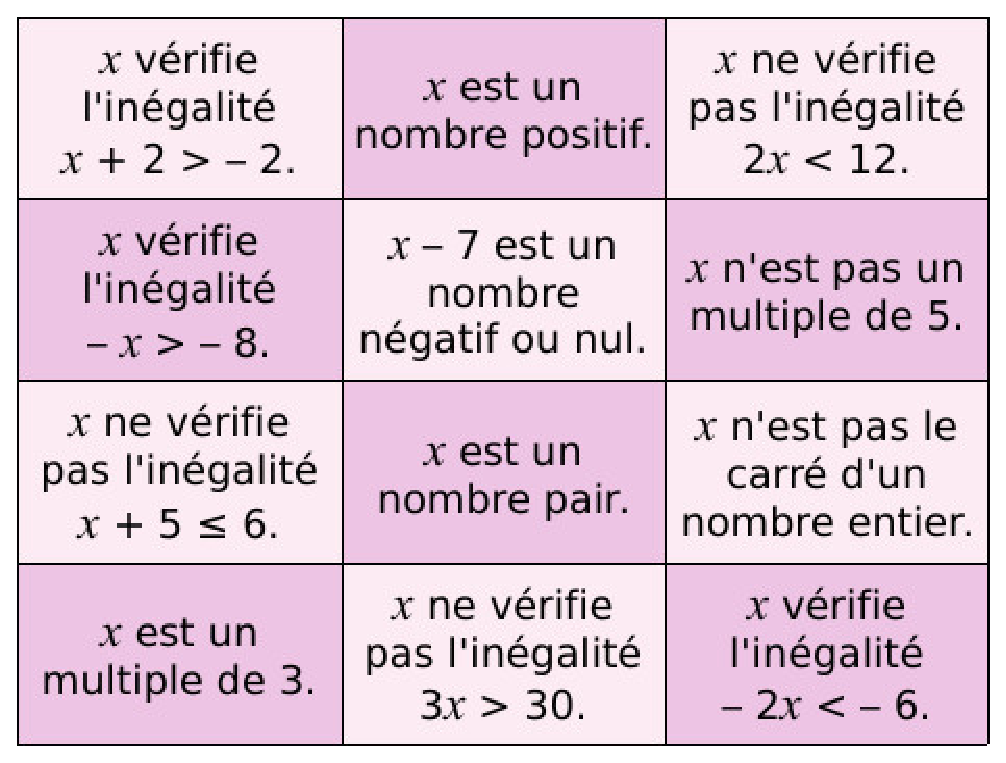
\includegraphics[width=.6\linewidth]{EqEA05}
\end{center}

% texte du carré (image ci-dessus)
%x vérifie l'inégalité
%x + 2 > – 2.
%x est un nombre positif.
%x ne vérifie pas l'inégalité
%2x < 12.
%x vérifie l'inégalité
%– x > – 8.
%x – 7 est un nombre  négatif ou nul.
%x n'est pas un multiple de 5.
%x ne vérifie pas l'inégalité
%x + 5 ≤ 6.
%x est un nombre pair.
%x n'est pas le carré d'un nombre entier.
%x est un multiple de 3.
%x ne vérifie pas l'inégalité 3x > 30.
%x vérifie l'inégalité – 2x < – 6.

\item Est-ce que tous les indices sont nécessaires pour trouver la valeur de $x$ ? Trouvez un nombre minimum d'indices qui permettent à eux seuls de déterminer $x$.


\vspace{1em}\textbf{2\up{e} Partie : Inventez vos indices}\vspace{1em}



\item Dans votre groupe, choisissez un nombre entier et inventez une liste de douze indices qui permettent de déterminer le nombre, en vous inspirant de la première partie. Tout comme dans la première partie, six indices au moins doivent utiliser une inégalité et aucun indice ne doit permettre de trouver immédiatement le nombre.
\item Fabriquez un jeu de quinze cartes avec vos indices. Recommencez l'opération avec un nouveau nombre. Vous aurez donc construit deux jeux de cartes.

\vspace{1em}\textbf{3\up{e} Partie : Jouez !}\vspace{1em}

\item Utilisez un jeu de cartes construit par un autre groupe. Un joueur distribue les cartes de manière à ce que chacun en ait le même nombre.
\begin{itemize}
    \item Le joueur à la gauche du donneur commence à jouer. C'est le détective. Il étudie ses cartes et propose à voix haute un nombre qui, selon lui, peut être le nombre mystère. Les autres joueurs étudient leurs cartes.
    \item Si un joueur trouve dans son jeu un indice qui prouve que le nombre choisi n'est pas le nombre mystère, il dit : \og Erreur ! \fg et montre son indice au détective.
    \item C'est alors le joueur à gauche du détective qui devient détective à son tour. Si aucun joueur n'a d'indice qui prouve que le nombre choisi n'est pas le nombre mystère, le détective a gagné.
\end{itemize}
\end{enumerate}
\end{TP}

